\documentclass[../piano-di-progetto.tex]{subfiles}
\begin{document}

\subsection{Verifica e collaudo}
Il periodo di validazione e collaudo inizia il 2020-06-19, dopo la revisione di avanzamento, e termina il giorno 2020-07-20 con la revisione di accettazione. 

\subsubsection{Ruoli}
Durante questa macro, viene richiesta la presenza dei seguenti ruoli:
\begin{itemize}
    \item Responsabile;
    \item Amministratore;
    \item Progettista;
    \item Programmatore;
    \item Verificatore.
\end{itemize}

\subsubsection{Attività}
Per semplicità, questa macro viene suddivisa in periodi:

\begin{itemize}
    \item \textbf{I periodo (2020-06-11 - 2020-06-17)}:
        \begin{itemize}
            \item \textbf{Preparazione della presentazione};
            \textbf{Verifica}.
        \end{itemize}
    \item \textbf{II periodo (2020-06-18 - 2020-06-28)}:
        \begin{itemize}
            \item \textbf{Normazione}: revisione e aggiornamento delle norme;
            \item \textbf{Pianificazione}: revisione e aggiornamento della pianificazione;
            \item \textbf{Qualità}: revisione e aggiornamento della pianificazione di qualità.
        \end{itemize}
    \item \textbf{III periodo (2020-06-29 - 2020-07-12)}:
        \begin{itemize}
            \item \textbf{Codifica}: rilascio della versione finale;
            \item Stesura finale del manuale;
            \item Stesura finale del consultivo;
            \item Verifica e collaudo finale.
        \end{itemize}
    \item \textbf{IV periodo (2020-07-13 - 2020-07-19}:
        \begin{itemize}
            \item Preparazione della presentazione;
            \item Verifica.
        \end{itemize}
\end{itemize}

\newpage
\begin{landscape}
    \begin{figure}[H]
        \centering
        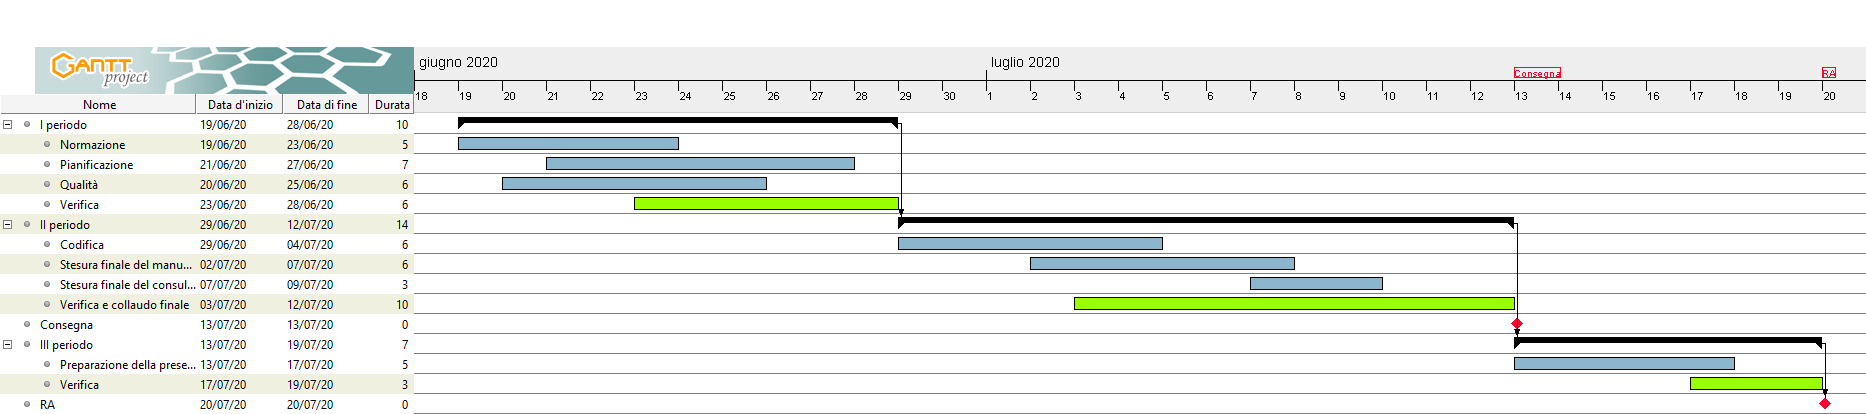
\includegraphics[width=24cm]{img/verifica.png}
        \caption{Diagramma attività nel periodo di verifica e collaudo}
      \end{figure}
\end{landscape}


\end{document}
